\chapter{\IfLanguageName{dutch}{Proof of concept en praktijktest}{Proof of concept and field tests}}
\label{ch:poc}
Na de literatuurstudie, requirementsanalyse en vergelijkende evaluatie van bestaande AI-systemen, vormt dit hoofdstuk een belangrijke schakel in het beantwoorden van de centrale onderzoeksvraag. Hierin wordt het geselecteerde AI-systeem geïmplementeerd in een reële context bij volleybalclub Lindemans Aalst als een proof of concept (PoC).

Deze fase heeft tot doel om de theoretische meerwaarde van het systeem in de praktijk te valideren. Tijdens trainingen en wedstrijden wordt geëvalueerd of het systeem voldoet aan de functionele en technische vereisten zoals geformuleerd in de voorgaande fases. Hierbij wordt bijzondere aandacht besteed aan de gebruiksvriendelijkheid, de nauwkeurigheid van dataverzameling, de snelheid van verwerking en de integratie in de bestaande werkwijze van de club.

Het oorspronkelijke plan voorzag een praktijktestperiode van twee weken. Echter, aangezien het volleybalseizoen onverwacht tot een einde kwam tijdens het midden van deze fase, kon de proof of concept slechts tijdens twee resterende wedstrijden worden uitgevoerd. Ondanks deze beperkte testperiode bood dit toch waardevolle inzichten in de toepasbaarheid en prestaties van het AI-systeem in een wedstrijdcontext.

Door de prestaties van het geautomatiseerde systeem te vergelijken met handmatig geregistreerde gegevens en door feedback van coaches en staf te verzamelen, wordt nagegaan of het AI-systeem daadwerkelijk een significante meerwaarde kan bieden voor de werking van de club. De inzichten uit deze praktijktest vormen een essentiële basis voor het formuleren van aanbevelingen omtrent een bredere implementatie op lange termijn.

\section{Kwartfinale Play-offs - 16/4/2025}
\subsection{Vergelijking van de statistieken}
\subsubsection{Set 1 - Greenyard Maaseik}
\label{sec:PL1_Greenyard1}
Voor de opslagen van de eerste set van Greenyard Maaseik worden tabellen \ref{tab:PL1ServeMaaseikMan1} en \ref{tab:PL1ServeMaaseikAI1} bekeken. De beoordeling van de opslag is op een andere wijze gedaan dan bij de manuele invoer. Bij de manuele invoer wordt er gebruik gemaakt van tekens, terwijl bij de AI-invoer gebruik wordt gemaakt van cijfers. Bij de opslag komt het teken \# overeen met 0, + en / met 1, ! met 2, - en = met 3.

Hier valt op dat de goede opslagen door beide in deze set niet zijn genoteerd. De AI-invoer heeft de opslagen meer verdeeld onder score 1 en 2. Terwijl de manuele invoer enkel score 1 of 3 heeft gegeven. De scouter is dus kritischer in zijn beoordeling van de opslag.

\begin{table}[ht!]
    \centering
    \scriptsize
    \begin{tabular}{|l|c|c|c|c|c|c|c|c|c|}
      \hline
      \textbf{Speler} & *E\% & Tot & = & / & - & ! & + & \# \\ \hline
      Samuel Fafchamps & 0\% & 3 & 1 &  & 1 &  & 1 &  \\ 
      Renet Vancker & 0\% & 1 &  &  & 1 &  &  &  \\ 
      Jolan Cox  & 33\% & 3 & 1 &  &  &  & 2 &  \\ 
      Dawid Pawlun  & -100\% & 1 & 1 &  &  &  &  &  \\ 
      Miquel Angel Fornés & 75\% & 4 &  &  & 1 &  & 3 &  \\
      Hampus Ekstrand & 75\% & 4 &  & 1 & 1 &  & 2 &  \\
      Pierre Perin & 100\% & 3 &  &  &  &  & 3 &  \\ \hline
    \end{tabular}
    \caption[Manueel ingevoerde opslagstatistieken voor Greenyard Maaseik in set 1]{\label{tab:PL1ServeMaaseikMan1}Manueel ingevoerd opslag statistieken voor Greenyard Maaseik in set 1.}
\end{table}

\begin{table}[ht!]
  \centering
  \scriptsize
  \begin{tabular}{|l|c|c|c|c|c|c|c|c|c|c|c|c|} \hline
    \textbf{Speler} & SA & SE & TA & Pct & Eff & Rtg & 0 & 1 & 2 & 3 \\ \hline
    Samuel Fafchamps &  & 1 & 3 & 67 & -0.33 & 2.33 &  & 1 &  & 2  \\
    Renet Vancker &  &  & 1 & 100 & 0.00 & 3.00 &  &  &  & 1  \\
    Jolan Cox &  & 1 & 3 & 67 & -0.33 & 2.00 &  & 1 & 1 & 1 \\
    Dawid Pawlun &  & 1 & 1 & 0 & -1 & 3.00 &  &  &  & 1 \\
    Miquel Angel Fornés &  &  & 4 & 100 & 0.00 & 1.33 &  & 2 & 1 & \\
    Hampus Ekstrand &  &  & 4 & 100 & 0.00 & 1.00 &  & 3 &  & \\
    Pierre Perin &  &  & 3 & 100 & 0.00 & 1.33 &  & 2 & 1 & \\ \hline
  \end{tabular}
  \caption[Opslagstatistieken gemaakt door Balltime AI voor Greenyard Maaseik in set 1]{\label{tab:PL1ServeMaaseikAI1}Opslag statistieken gemaakt door Balltime AI voor Greenyard Maaseik in set 1.}
\end{table}

De recepties worden in tabellen \ref{tab:PL1ReceiveMaaseikMan1} en \ref{tab:PL1ReceiveMaaseikAI1} weergegeven. De manuele invoer heeft de recepties beoordeeld met de tekens \# overeen met 3, + en / met 2, ! met 1, - en = met 0.

Bij de receptie zijn er grote verschillen aanwezig tussen de manuele invoer en de AI-invoer. Er is één receptie van Landon Douglas Currie die door de AI-invoer niet kon beoordeeld worden, maar ook hier kan er geconstateerd worden dat de manuele invoer veel kritischer is in zijn beoordeling. 

\begin{table}[ht!]
    \centering
    \scriptsize
    \begin{tabular}{|l|c|c|c|c|c|c|c|c|c|}
        \hline
        \textbf{Speler} & *E\% & Tot & = & / & - & ! & + & \# \\ \hline
        Landon Douglas Currie & 38\% & 8 & 1 & 1 &  & 1 & 2 & 3 \\ 
        Hampus Ekstrand & 33\% & 3 &  &  &  & 2 & 1 &  \\ 
        Pierre Perin & 88\% & 8 &  &  &  & 1 & 2 & 5  \\ \hline
    \end{tabular}
    \caption[Manueel ingevoerde receptiestatistieken voor Greenyard Maaseik in set 1]{\label{tab:PL1ReceiveMaaseikMan1}Manueel ingevoerd receptie statistieken voor Greenyar Maaseik in set 1.}
\end{table}

\begin{table}[ht!]
  \centering
  \scriptsize
  \begin{tabular}{|l|c|c|c|c|c|c|c|c|c|} \hline
    \textbf{Speler} & 3 & 2 & 1 & 0 & TA & ? & Pass\% & Perfect PP\% & Good GP\% \\ \hline
    Thomas Neyens &  &  & 1 &  & 1 &  & 1.00 & 0 & 0  \\
    Landon Douglas Currie & 4 & 1 & 1 &  & 7 & 1 & 2.50 & 67 & 83 \\
    Hampus Ekstrand & 2 & 1 &  & 1 & 4 &  & 2.00 & 50 & 75 \\
    Pierre Perin & 5 & 1 & 2 &  & 8 &  & 2.38 & 62 & 75 \\ \hline
  \end{tabular}
  \caption[Receptie statistieken gemaakt door Balltime AI voor Greenyard Maaseik in set 1]{\label{tab:PL1ReceiveMaaseikAI1}Receptie statistieken gemaakt door Balltime AI voor Greenyard Maaseik in set 1.}
\end{table}

De spelverdeling wordt weergegeven in tabellen \ref{tab:PL1SetMaaseikMan1} en \ref{tab:PL1SetDigMaaseikAI1}. Over het algemeen zijn de hoeveelheden van de spelverdeling correct, bij één speler is er een verschil van 1 bij de AI-invoer. De kwaliteit van de set wordt bij de AI niet beoordeeld, waardoor geen verdere vergelijking mogelijk is.

Bij de verdeding, tabel \ref{tab:PL1DigMaaseikMan1} en \ref{tab:PL1SetDigMaaseikAI1}, zijn er duidelijke verschillen te zien. Dig Error (DE) komt overeen met een = bij de manuele invoer. Bij 2 spelers komt dit perfect overeen met de manuele invoer, bij de andere is er echter wel een verschil.  Zij hebben meer of minder verdedigingen gekregen door de AI.

\begin{table}[ht!]
    \centering
    \scriptsize
    \begin{tabular}{|l|c|c|c|c|c|c|c|c|c|}
        \hline
        \textbf{Speler}& *E\% & Tot & = & / & - & ! & + & \# \\ \hline
        Renet Vancker  & 100\% & 7 &  &  &  &  & 6 & 1  \\
        Jolan Cox  & 100\% & 1 &  &  &  &  & 1 &  \\ 
        Dawid Pawlun  & 100\% & 14 &  &  &  &  & 13 & 1  \\ 
        Pierre Perin & 100\% & 2 &  &  &  &  & 2 & \\ \hline
    \end{tabular}
    \caption[Manueel ingevoerde spelverdelingsstatistieken gemaakt voor Greenyard Maaseik in set 1]{\label{tab:PL1SetMaaseikMan1}Manueel ingevoerde spelverdeling statistieken gemaakt voor Greenyard Maaseik in set 1.}
\end{table}

\begin{table}[ht!]
    \centering
    \scriptsize
    \begin{tabular}{|l|c|c|c|c|c|c|c|c|c|}
        \hline
        \textbf{Speler}  & *E\% & Tot & = & / & - & ! & + & \# \\ \hline
        Jolan Cox & 0\% & 2 & 1 &  & 1 &  &  &  \\ 
        Landon Douglas Currie & 100\% & 1 &  &  &  &  & 1 &  \\ 
        Dawid Pawlun & 100\% & 1 &  &  &  &  & 1 &  \\ 
        Miquel Angel Fornés & 100\% & 1 &  &  &  &  & 1 &  \\ 
        Hampus Ekstrand & 0\% & 4 & 3 &  & 1 &  &  &  \\ 
        Pierre Perin & 50\% & 2 & 1 &  &  &  & 1 &  \\ \hline
    \end{tabular}
    \caption[Manueel ingevoerde verdedigingsstatistieken gemaakt voor Greenyard Maaseik in set 1]{\label{tab:PL1DigMaaseikMan1}Manueel ingevoerde verdediging statistieken gemaakt voor Greenyard Maaseik in set 1.}
\end{table}

\begin{table}[ht!]
  \centering
  \scriptsize
  \begin{tabular}{|l|c|c|c|c|c|c|c|}  \hline
    \textbf{Speler} & Ast & TA & SE & A/S & PCT & DS & DE \\ \hline
    Renet Vancker & 4 & 7 &  & 4.00 & 57 &  &  \\
    Thomas Neyens &  &  &  &  &  & 1 &  \\
    Jolan Cox &  & 1 &  & 0.00 & 0 & 1 & 1 \\
    Landon Douglas Currie &  &  &  &  &  & 1 &  \\
    Dawid Pawlun & 6 & 13 &  & 6.00 & 46 & 1 &  \\
    Miquel Angel Fornés &  &  &  &  &  & 1 & 1 \\
    Hampus Ekstrand &  &  &  &  &  & 3 & 1 \\
    Pierre Perin &  & 2 &  & 0.00 & 0 & 1 &  \\ \hline
  \end{tabular}
  \caption[Spelverdeling- en verdedigingsstatistieken gemaakt door Balltime AI voor Greenyard Maaseik in set 1]{\label{tab:PL1SetDigMaaseikAI1}Spelverdeling en verdediging statistieken gemaakt door Balltime AI voor Greenyard Maaseik in set 1.}
\end{table}

Bij de aanval (tabel \ref{tab:PL1AttMaaseikMan1} en \ref{tab:PL1AttBlockMaaseik1}) is het totaal aantal aanvallen gelijk bij iedereen behalve twee spelers. Zij hebben 1 en 2 aanvallen minder.

Bij de blokstatistieken (tabel \ref{tab:PL1BlockMaaseikMan1} en \ref{tab:PL1AttBlockMaaseik1}) wordt er op een volledig andere manier naar gekeken. De AI geeft statistieken waar de speler deel kan zijn van een éénmans- of een meermansblock. Dit is bij de manuele invoer niet het geval. Hierdoor geeft de AI dus eigenlijk ook geen blokpunten aan de spelers. Ookal is dit wel belangrijke informatie.

De aanvallen en blocks worden door de AI niet beoordeeld op kwaliteit.

\begin{table}[ht!]
    \centering
    \scriptsize
    \begin{tabular}{|l|c|c|c|c|c|c|c|c|c|}
        \hline
        \textbf{Speler} & *E\% & Tot & = & / & - & ! & + & \# \\ \hline
        Samuel Fafchamps & 75\% & 4 &  &  &  &  & 1 & 3 \\ 
        Jolan Cox & -20\% & 5 & 2 & 1 &  &  &  & 2 \\ 
        Dawid Pawlun  & 100\% & 2 & 1 &  &  &  &  & 2 \\ 
        Miquel Angel Fornés & 60\% & 5 &  &  &  &  & 2 & 3 \\
        Hampus Ekstrand & 25\% & 4 &  &  &  & 1 & 2 & 1 \\ 
        Pierre Perin & -17\% & 6 & 1 & 1 & 1 & 1 & 1 & 1 \\ \hline
    \end{tabular}
    \caption[Manueel ingevoerde aanvalsstatistieken gemaakt Greenyard Maaseik in set 1]{\label{tab:PL1AttMaaseikMan1}Manueel ingevoerde aanval statistieken gemaakt voor GreenyardMaaseik in set 1.}
\end{table}

\begin{table}[ht!]
    \centering
    \scriptsize
    \begin{tabular}{|l|c|c|c|c|c|c|c|c|c|}
        \hline
        \textbf{Speler} & *E\% & Tot & = & / & - & ! & + & \# \\ \hline
        Samuel Fafchamps & 0\% & 2 &  &  &  & 1 & 1 &  \\ 
        Jolan Cox & 100\% & 1 &  &  &  &  &  & 1 \\ 
        Dawid Pawlun & -100\% & 2 & 2 &  &  &  &  &  \\ 
        Hampus Ekstrand & 0\% & 2 & 1 &  &  &  &  & 1 \\ \hline
    \end{tabular}
    \caption[Manueel ingevoerde blokstatistieken gemaakt Greenyard Maaseik in set 1]{\label{tab:PL1BlockMaaseikMan1}Manueel ingevoerde blok statistieken gemaakt voor GreenyardMaaseik in set 1.}
\end{table}

\begin{table}[ht!]
  \centering
  \scriptsize
  \begin{tabular}{|l|c|c|c|c|c|c|c|c|c|c|c|} \hline
    \textbf{Speler} & K & E & TA & Atk\% & Kill\% & K/S & Error\% & BS & BA & BE \\ \hline
    Samuel Fafchamps & 3 &  & 4 & 0.75 & 75 & 3 & 0 &  &  & \\
    Jolan Cox & 2 & 3 & 6 & -0.17 & 33 & 2 & 50 & 1 &  &  \\
    Dawid Pawlun &   &   &   &   &   &   &   & 1 &  &   \\
    Miquel Angel Fornés & 3 &  & 5 & 0.60 & 6. & 3 &  & 1 & 1 & \\
    Hampus Ekstrand & 1 &  & 4 & 0.25 & 25 & 1 & 1 &  & 1 & \\
    Pierre Perin & 1 & 2 & 6 & -0.17 & 17 & 1 & 33 &  &   &  \\ \hline
    \end{tabular}
  \caption[Aanval en blokstatistieken gemaakt door Balltime AI voor Greenyard Maaseik in set 1]{\label{tab:PL1AttBlockMaaseik1}Aanval en blok statistieken gemaakt door Balltime AI voor Greenyard Maaseik in set 1.}
\end{table}

\subsubsection{Set 2 - Lindemans Aalst}
\label{sec:PL1_Aalst2}
In de tabellen \ref{tab:PL1ServeAalstMan2} en \ref{tab:PL1ServeAalstAI2} zijn de serve statistieken van Lindemans Aalst in set 2 weergegeven. De eerste tabel toont de manueel ingevoerde statistieken, terwijl de tweede tabel de statistieken toont die door Balltime AI zijn gegenereerd. De serve statistieken zijn onderverdeeld in verschillende categorieën, zoals het aantal serves, het percentage fouten en de effectiviteit van de serve. De beoordeling van de opslag is op een andere wijze gedaan dan bij de manuele invoer. Bij de manuele invoer wordt er gebruik gemaakt van tekens, terwijl bij de AI-invoer gebruik wordt gemaakt van cijfers. Bij de opslag komt het teken \# overeen met 0, + en / met 1, ! met 2, - en = met 3. Eerst en vooral valt op dat de AI niet alle recepties heeft beoordeeld. Daarnaast kan besloten worden dat zowel de AI als de scouter de perfecte receptie gelijk beoordelen. Bij de andere vergelijking speelt de mening van de scouter een grote rol. Bij score 1 zijn er grote verschillen, enkel bij speler Max Schulz is er een zelfde hoeveelheid. Score 2 werd door de scouter niet aan een opslag gegeven, maar de AI heeft dit wel gedaan. De slechte recepties worden ook opnieuw anders beoordeeld.

\begin{table}[ht!]
  \centering
  \scriptsize
    \begin{tabular}{|l|c|c|c|c|c|c|c|c|} \hline
      \textbf{Speler} & *E\% & Tot & = & / & - & ! & + & \# \\ \hline
      Hiago Crins & 33 & 3 &  &  & 2 &  & 1 & \\ 
      Timo Lohmus & 25 & 4 & 1 &  & 1 & & 1 & 1 \\ 
      Max Schulz & 0 & 3 & 1 &  & 1 &  & 1 &  \\ 
      Mihkel Varblane & 100 & 2 &  &  &  &  & 2 & \\
      Alvaro Gimeno Rubio & 71 & 7 & 1 & 1 &  &  & 4 & 1\\
      Lucas Lorente López & 0 & 3 &  &  & 3 &  &  &  \\ \hline
  \end{tabular}
  \caption[Manueel ingevoerd opslag statistieken voor Lindemans Aalst in set 2]{\label{tab:PL1ServeAalstMan2}Manueel ingevoerd opslag statistieken voor Lindemans Aalst in set 2.}
\end{table}

\begin{table}[ht!]
  \centering
  \scriptsize
  \begin{tabular}{|l|c|c|c|c|c|c|c|c|c|c|c|c|} \hline
    \textbf{Speler} & SA & SE & TA & Pct (\%) & Eff & Rtg & 0 & 1 & 2 & 3 \\ \hline
    Timo Lohmus & 1 & 1 & 4 & 75 & 0 & 1.75 & 1 & & 2 & 1 \\
    Max Schulz & 0 & 1 & 3 & 67 & -0.33 & 2.33 &  & 1 &  & 2 \\
    Hiago Crins & 0 & 0 & 3 & 100 & 0 & 1.67 &  & 2 &  & 1 \\
    Mihkel Varblane & 0 & 0 & 2 & 100 & 0 & 1 &  & 1 &  &   \\
    Alvaro Gimeno Rubio & 1 & 1 & 7 & 86 & 0 & 1.6 & 1 & 2 &  & 2  \\
    Robbe Ponseele & 1 & 1 & 2 & 50 & 0 & 1.5 & 1 &  &  & 1  \\
    Lucas Lorente López & 0 & 0 & 3 & 1 & 0 & 2.33 &  & 1 &  & 2  \\ \hline
  \end{tabular}
  \caption[Opslag statistieken gemaakt door Balltime AI voor Lindemans Aalst in set 2]{\label{tab:PL1ServeAalstAI2}Opslag statistieken gemaakt door Balltime AI voor Lindemans Aalst in set 2.}
\end{table}

In de tabellen \ref{tab:PL1ReceiveAalstMan2} en \ref{tab:PL1ReceiveAalstAI2} zijn de receptie statistieken van Lindemans Aalst in set 2 weergegeven. De eerste tabel toont de manueel ingevoerde statistieken, terwijl de tweede tabel de statistieken toont die door Balltime AI zijn gegenereerd. De receptie statistieken zijn onderverdeeld in verschillende categorieën, zoals het aantal recepties, het percentage fouten en de effectiviteit van de receptie. De beoordeling van de receptie is op een andere wijze gedaan dan bij de manuele invoer. Bij de manuele invoer wordt er gebruik gemaakt van tekens, terwijl bij de AI-invoer gebruik wordt gemaakt van cijfers. Bij de receptie komt het teken \# overeen met 3, + en / met 2, ! met 1, - en = met 0. De AI heeft maar 1 opslag niet beoordeeld. Hier valt direct op dat de AI de recepties positiever heeft beoordeeld dan de scouter. Dit is te zien bij de score 0, waar de AI geen recepties heeft gegeven en de scouter 6. Score 3 werd door de scouter aan 1 opslag gegeven, maar de AI gaf dit aan 5.

\begin{table}[ht!]
  \centering
  \scriptsize
    \begin{tabular}{|l|c|c|c|c|c|c|c|c|c|}
      \hline
      \textbf{Speler} & *E\% & Tot & = & / & - & ! & + & \# \\ \hline
      Bert Dufraing  & 50 & 2 &  &  & 1 &  &  & 1 \\ 
      Timo Lohmus  & 29 & 7 &  & & 2 & 3 & 2 &    \\
      Max Schulz  & 25 & 8 &  &  & 3 & 3 & 1 &   \\ \hline
  \end{tabular}
  \caption[Manueel ingevoerd receptie statistieken voor Lindemans Aalst in set 2]{\label{tab:PL1ReceiveAalstMan2}Manueel ingevoerd receptie statistieken voor Lindemans Aalst in set 2.}
\end{table}

\begin{table}[ht!]
  \centering
  \scriptsize
  \begin{tabular}{|l|c|c|c|c|c|c|c|c|c|} \hline
    \textbf{Speler} & 3 & 2 & 1 & 0 & TA & ? & Pass\% & Perfect PP\% (\%) & Good GP\% (\%) \\ \hline
    Bert Dufraing & 1 &  & 1 &  & 2 &  & 2.00 & 50 & 50 \\
    Timo Lohmus & 1 & 3 & 3 &  & 7 &  & 1.71 & 14 & 58 \\
    Max Schulz & 3 & 3 & 2 &  & 8 &  & 2.12 & 38 & 75 \\  \hline
  \end{tabular}
  \caption[Receptie statistieken gemaakt door Balltime AI voor Lindemans Aalst in set 2]{\label{tab:PL1ReceiveAalstAI2}Receptie statistieken gemaakt door Balltime AI voor Lindemans Aalst in set 2.}
\end{table}

Tabel \ref{tab:PL1SetAalstMan2}, \ref{tab:PL1DigAalstMan2} en \ref{tab:PL1SetDigAalstAI2} geven de setting en verdediging statistieken van Lindemans Aalst in set 2 weer. De eerste tabel toont de manueel ingevoerde statistieken van de spelverdeling, terwijl de derde tabel de statistieken toont die door Balltime AI zijn gegenereerd. De setting statistieken zijn onderverdeeld in verschillende categorieën, zoals het aantal sets, het percentage fouten en de effectiviteit van de set. Setter Lucas Lorente López heeft in deze set 19 sets gegeven volgens de scouter en 18 volgens de AI. Bij de andere spelers is dit aantal hetzelfde tussen AI en de manuele invoer. Ook hier is er een verschil op de weergave van de statistieken. = komt overeen met een Serve Error (SE). Dit is bij beide hetzelfde. De kwaliteit van de set wordt bij de AI niet beoordeeld, waardoor geen verdere vergelijking mogelijk is.

Bij de verdediging is er een groot verschil tussen de AI en de scouter. De AI heeft verschillende verdedigingen niet erkend, terwijl de scouter dit wel heeft gedaan. Dit is te zien bij bijvoorbeeld Hiago Crins, die 3 verdedigingen heeft gegeven, maar de AI heeft er maar 1 erkend.

\begin{table}[ht!]
  \centering
  \scriptsize
    \begin{tabular}{|l|c|c|c|c|c|c|c|c|c|} \hline
      \textbf{Speler} & *E\% & Tot & = & / & - & ! & + & \# \\ \hline
      Timo Lohmus & 0 & 2 & 1 &  &  &  & 1 &   \\
      Max Schulz & 50 & 2 &  &  & 1 & & 1 &  \\
      Alvaro Gimeno Rubio  & 50 & 2 &  &  & 1 &  & 1 &   \\ 
      Lucas Lorente López  & 100 & 19 &  &  &  &  & 19 &  \\ \hline
  \end{tabular}
  \caption[Manueel ingevoerde spelverdeling statistieken gemaakt voor Lindemans Aalst in set 2]{\label{tab:PL1SetAalstMan2}Manueel ingevoerde spelverdeling statistieken gemaakt voor Lindemans Aalst in set 2.}
\end{table}

\begin{table}[ht!]
  \centering
  \scriptsize
    \begin{tabular}{|l|c|c|c|c|c|c|c|c|c|}
      \hline
      \textbf{Speler} & *E\% & Tot & = & / & - & ! & + & \# \\ \hline
      Hiago Crins & 0 & 3 & 1 &  &  & 1 & 1 &  \\ 
      Bert Dufraing & 100 & 2 &  &  &  &  & 2 &  \\
      Timo Lohmus & 100 & 1 &  &  &  &  & 1 &  \\
      Max Schulz & 67 & 3 & 1 & 2 &  &  &  &  \\
      Mihkel Varblane & 67 & 3 & 1 &  &  &  & 2 &  \\
      Alvaro Gimeno Rubio & 100 & 2 &  & 1 &  & 1 &  &  \\
      Lucas Lorente López & 0 & 1 &  &  & 1 &  &  &  \\ \hline
  \end{tabular}
  \caption[Manueel ingevoerde verdediging statistieken gemaakt voor Lindemans Aalst in set 2]{\label{tab:PL1DigAalstMan2}Manueel ingevoerde verdediging statistieken gemaakt voor Lindemans Aalst in set 2.}
\end{table}

\begin{table}[ht!]
  \centering
  \scriptsize
  \begin{tabular}{|l|c|c|c|c|c|c|c|} \hline
    \textbf{Speler} & Ast & TA & SE & A/S & PCT (\%) & DS & DE \\ \hline
    Hiago Crins &  &  &  &  &  & 1 &  \\
    Bert Dufraing &  &  &  &  &  & 1 &  \\ 
    Timo Lohmus & 1 & 2 & 1 & 1.00 & 50 & 1 &  \\
    Max Schulz & 1 & 2 &  & 1.00 & 50 & 1 & 1 \\
    Mihkel Varblane &  &  &  &  &  & 2 &  \\
    Alvaro Gimeno Rubio & 0 & 2 &  & 0.00 & 0 & 3 &  \\
    Lucas Lorente López & 10 & 18 &  & 10.00 & 56 & 1 &  \\ \hline
  \end{tabular}
  \caption[Spelverdeling en verdediging statistieken gemaakt door Balltime AI voor Lindemans Aalst in set 2]{\label{tab:PL1SetDigAalstAI2}Spelverdeling en verdediging statistieken gemaakt door Balltime AI voor Lindemans Aalst in set 2.}
\end{table}

Bij de aanval (tabel \ref{tab:PL1AttAalstMan2} en \ref{tab:PL1AttBlockAalstAI2}) is het totaal aantal aanvallen gelijk bij iedereen behalve één speler. Hij heeft een aanval minder gekregen door de AI. 

Bij de block statistieken (tabel \ref{tab:PL1BlockAalstMan2} en \ref{tab:PL1AttBlockAalstAI2}) wordt er op een volledig andere manier naar gekeken. De AI geeft statistieken waar de speler deel kan zijn van een éénmans- of een meermansblock. Dit is bij de manuele invoer niet het geval. Hierdoor geeft de AI dus eigenlijk ook geen blockpunten aan de spelers. Ookal is dit wel belangrijke informatie.

De aanvallen en blocks worden door de AI niet beoordeeld op kwaliteit.

\begin{table}[ht!]
  \centering
  \scriptsize
    \begin{tabular}{|l|c|c|c|c|c|c|c|c|c|}
      \hline
      \textbf{Speler} & *E\% & Tot & = & / & - & ! & + & \# \\ \hline
      Hiago Crins  & 0 & 1 &  &  &  &  & 1 &  \\ 
      Timo Lohmus  & 17 & 6 & 1 &  & 1 & 1 & 1 & 2 \\ 
      Max Schulz  & 22 & 9 & 1 & 2 &  & 1 & 0 & 5\\
      Mihkel Varblane  & 100 & 2 &  &  &  &  &  & 2 \\ 
      Alvaro Gimeno Rubio & 29 & 7 & 1 & 1 &  &  & 1 & 4 \\ \hline 
  \end{tabular}
\caption[Manueel ingevoerde aanval statistieken gemaakt Lindemans Aalst in set 2]{\label{tab:PL1AttAalstMan2}Manueel ingevoerde aanval statistieken gemaakt voor Lindemans Aalst in set 2.}
\end{table}

\begin{table}[ht!]
  \centering
  \scriptsize
    \begin{tabular}{|l|c|c|c|c|c|c|c|c|c|}
      \hline
      \textbf{Speler} & *E\% & Tot & = & / & - & ! & + & \# \\ \hline
      Hiago Crins & -25 & 4 & 1 &  & 2 & 1 &  &  \\ 
      Max Schulz & 0 & 1 &  &  &  & 1 &  & \\
      Mihkel Varblane & 33 & 3 &  &  & 1 &  & 1 & 2 \\
      Alvaro Gimeno Rubio & -50 & 2 &  & &  &  & 1 &  \\
      Lucas Lorente López & 0 & 1 &  &  & 1 &  &  &  \\ \hline
  \end{tabular}
\caption[Manueel ingevoerde block statistieken gemaakt Lindemans Aalst in set 2]{\label{tab:PL1BlockAalstMan2}Manueel ingevoerde block statistieken gemaakt voor Lindemans Aalst in set 2.}
\end{table}

\begin{table}[ht!]
  \centering
  \scriptsize
  \begin{tabular}{|l|c|c|c|c|c|c|c|c|c|c|c|} \hline
    \textbf{Speler} & K & E & TA & Atk\% & Kill\%  & Error\% & BS & BA & BE & B/S \\ \hline
    Hiago Crins & & & 1 & 0.00 & 0  & 0 & 1 & 1 & & 1.00 \\
    Timo Lohmus & 3 & 1 & 6 & 0.33 & 50  & 17 &  &  & & \\
    Max Schulz & 5 & 3 & 9 & 0.22 & 56  & 33 &  & 2 & & 0.00 \\
    Mihkel Varblane & 2 & 0 & 2 & 1.00 & 100  & 0 & 1 & 1 & & 1.00 \\
    Alvaro Gimeno Rubio & 3 & 2 & 6 & 0.17 & 50  & 33 &  & 1 & & 0.00\\
    Lucas Lorente López &  &  &  &  &  &  &  & 1 & & 0.00 \\ \hline
  \end{tabular}
  \caption[Aanval en block statistieken gemaakt door Balltime AI voor Lindemans Aalst in set 2]{\label{tab:PL1AttBlockAalstAI2}Aanval en block statistieken gemaakt door Balltime AI voor Lindemans Aalst in set 2.}
\end{table}

\subsubsection{Set 3 - Greenyard Maaseik}
\label{sec:PL1_Greenyard3}

Voor de opslagen worden tabellen \ref{tab:PL1ServeMaaseikMan3} en \ref{tab:PL1ServeMaaseikAI3} bekeken. De beoordeling van de opslag is op een andere wijze gedaan dan bij de manuele invoer. Bij de manuele invoer wordt er gebruik gemaakt van tekens, terwijl bij de AI-invoer gebruik wordt gemaakt van cijfers. Bij de opslag komt het teken \# overeen met 0, + en / met 1, ! met 2, - en = met 3.
Het aantal opslagen is bij beide hetzelfde getal. Ook de gemiste en perfecte opslagen zijn gelijk. De AI-invoer is echter veel minder kritisch dan de manuele invoer.

\begin{table}[ht!]
    \centering
    \scriptsize
    \begin{tabular}{|l|c|c|c|c|c|c|c|c|c|} \hline
        \textbf{Speler}& *E\% & Tot & = & / & - & ! & + & \#\\ \hline
        Samuel Fafchamps  & -33\% & 3 & 1 &  &  & 2 &  &  \\ 
        Jolan Cox  & -33\% & 3 & 2 &  & 1 &  &  &  \\ 
        Dawid Pawlun & 0\% & 2 &  &  & 2 &  &  &  \\
        Tijmen Bus & -100\% & 1 & 1 &  &  &  &  &  \\ 
        Miquel Angel Fornés & 100\% & 3 &  &  &  &  & 2 & 1 \\ 
        Hampus Ekstrand & 50\% & 2 &  &  & 1 &  &  & 1 \\ 
        Pierre Perin & 25\% & 4 & 1 &  & 1 &  &  & 2 \\ \hline
    \end{tabular}
    \caption[Manueel ingevoerde opslagstatistieken voor Greenyard Maaseik in set 3]{\label{tab:PL1ServeMaaseikMan3}Manueel ingevoerde opslagstatistieken voor Greenyard Maaseik in set 3.}
\end{table}

\begin{table}[ht!]
  \centering
  \scriptsize
  \begin{tabular}{|l|c|c|c|c|c|c|c|c|c|c|c|c|} \hline
    \textbf{Speler} & SA & SE & TA & Pct & Eff & Rtg & 0 & 1 & 2 & 3  \\ \hline
    Samuel Fafchamps &  & 1 & 3 & 67 & -0.33 & 2.33 &   &   & 2 & 1 \\
    Jolan Cox &  & 2 & 3 & 33 & -0.67 & 2.33 &   & 1 &   & 2 \\
    Dawid Pawlun &  &  & 2 & 100 & 0.00 & 1.50 &   & 1 & 1 &  \\
    Tijmen Bus &  & 1 & 1 & 0 & -1.00 & 3.00 &   & &   &  1 \\
    Miquel Angel Fornés & 1 &  & 3 & 100 & 0.33 & 1.33 & 1 & 1 &   & 1 \\
    Hampus Ekstrand & 1 &  & 2 & 100 & 0.50 & 1.00 & 1 &   & 1 &  \\
    Piere Perin & 2 & 1 & 4 & 75 & 0.25 & 1.5 & 2 &   &   & 2 \\ \hline
  \end{tabular}
  \caption[Opslagstatistieken gemaakt door Balltime AI voor Greenyard Maaseik in set 3]{\label{tab:PL1ServeMaaseikAI3}Opslagstatistieken gemaakt door Balltime AI voor Greenyard Maaseik in set 3.}
\end{table}

De recepties worden in tabellen \ref{tab:PL1ReceiveMaaseikMan3} en \ref{tab:PL1ReceiveMaaseikAI3} weergegeven. De manuele invoer heeft de recepties beoordeeld met de tekens \# overeen met 3, + en / met 2, ! met 1, - en = met 0. Op het eerste zicht valt op dat er een andere hoeveelheden recepties zijn geregisteerd bij sommige spelers. Opnieuw valt ook weer op dat de manuele invoer kritischer is dan de AI-invoer. Één opslag is ook niet gequoteerd geweest door de AI.

\begin{table}[ht!]
  \centering
  \scriptsize
  \begin{tabular}{|l|c|c|c|c|c|c|c|c|c|}
    \hline
    \textbf{Speler}& *E\% & Tot & = & / & - & ! & + & \#\\ \hline
    Andris Sirjakovs & 0\% & 2 &  &  &  & 2 &  &  \\ 
    Jolan Cox & -100\% & 1 &  & 1 &  &  &  &  \\
    Landon Douglas Currie & 60\% & 5 &  &  &  & 2 & 2 & 1 \\
    Tijmen Bus & -100\% & 1 &  & 1 &  &  &  &  \\ 
    Miquel Angel Fornés & 0\% & 1 &  &  & 1 &  &  &  \\ 
    Hampus Ekstrand & 17\% & 6 & 1 &  & 2 & 3 &  &  \\ 
    Pierre Perin & 29\% & 7 &  &  & 4 & 1 & 1 & 1 \\ \hline
  \end{tabular}
  \caption[Manueel ingevoerde receptiestatistieken voor Greenyard Maaseik in set 3]{\label{tab:PL1ReceiveMaaseikMan3}Manueel ingevoerde receptiestatistieken voor Greenyard Maaseik in set 3.}
\end{table}

\begin{table}[ht!]
  \centering
  \scriptsize
  \begin{tabular}{|l|c|c|c|c|c|c|c|c|c|} \hline
    \textbf{Speler} & 3 & 2 & 1 & 0 & TA & ? & Pass\% & Perfect PP\% & Good GP\% \\ \hline
    Andris Sirjakovs &  & 2 &  &  & 2 &  & 2 & 0 & 100 \\
    Landon Douglas Currie & 2 & 2 & 1 &  & 5 &  & 2.20 & 40 & 80 \\
    Tijmen Bus &  &  & 1 &  & 2 & 1 & 1.00 & 0 & 0 \\
    Miquel Angel Fornés &   &  & 1 &  & 1 &  & 1.00 & 0 & 0 \\
    Hampus Ekstrand &  & 2 & 3 & 1 & 6 &  & 1.17 & 0 & 33 \\
    Piere Perin & 1 & 1 & 4 &  & 6 &  & 1.50 & 17 & 33 \\ \hline
  \end{tabular}
  \caption[Receptiestatistieken gemaakt door Balltime AI voor Greenyard Maaseik in set 3]{\label{tab:PL1ReceiveMaaseikAI3}Receptiestatistieken gemaakt door Balltime AI voor Greenyard Maaseik in set 3.}
\end{table}

In tabellen \ref{tab:PL1SetMaaseikMan3} en \ref{tab:PL1SetDigMaaseikAI3} wordt de spelverdeling weergegeven. De hoeveelheden zijn hier zeer verschillend. Bij sommige spelers geeft de manuele invoer ze meer, bij andere dan weer meer door de AI. Volgens manuele invoer heeft Jolan Cox ook vijf keer aan spelverdeling gedaan, terwijl dit door AI geen enkele keer was. Dawid Pawlun heeft door de AI 17 keer aan spelverdeling gedaan, terwijl dit manueel maar 14 keer was. Dit is een verschil van 3. Dit is een groot verschil, maar het kan zijn dat de AI deze als spelverdeling heeft gezien, terwijl dit manueel niet zo was.

Ook bij de verdeding, tabel \ref{tab:PL1DigMaaseikMan3} en \ref{tab:PL1SetDigMaaseikAI3}, zijn er duidelijke verschillen te zien. Hier zijn er ook meerdere spelers die verschillende hoeveelheden verdedigingsacties hebben gekregen. Dit kan iets te maken hebben dat de verdediging buiten het beeld van de camera is gebeurd, waardoor de AI dit niet heeft kunnen registreren.

\begin{table}[ht!]
    \centering
    \scriptsize
    \begin{tabular}{|l|c|c|c|c|c|c|c|c|c|} \hline
        \textbf{Speler} & *E\% & Tot & = & / & - & ! & + & \# \\ \hline
        Samuel Fafchamps  & 100\% & 1 &  &  &  &  & 1 &  \\ 
        Renet Vancker & 100\% & 3 &  &  &  &  & 3 &  \\
        Jolan Cox & 100\% & 5 &  &  &  &  & 5 &  \\ 
        Landon Douglas Currie & 100\% & 1 &  &  &  &  & 1 &  \\ 
        Dawid Pawlun & 100\% & 14 &  &  &  &  & 11 & 3 \\ 
        Hampus Ekstrand & 100\% & 1 &  &  &  &  & 1 &  \\
        Pierre Perin & 100\% & 4 &  &  &  &  & 4 &  \\ \hline
    \end{tabular}
    \caption[Manueel ingevoerde spelverdelingsstatistieken voor Greenyard Maaseik in set 3]{\label{tab:PL1SetMaaseikMan3}Manueel ingevoerde spelverdeling statistieken voor Greenyard Maaseik in set 3.}
\end{table}

\begin{table}[ht!]
    \centering
    \scriptsize
    \begin{tabular}{|l|c|c|c|c|c|c|c|c|c|} \hline
        \textbf{Speler} & *E\% & Tot & = & / & - & ! & + & \#\\ \hline
        Renet Vancker & 0\% & 2 & 1 &  & 1 &  &  &  \\ 
        Jolan Cox & 75\% & 4 &  & 1 & 1 &  & 2 &  \\ 
        Landon Douglas Currie & 50\% & 2 &  &  & 1 &  & 1 &  \\ 
        Dawid Pawlun & 33\% & 3 &  &  & 2 &  & 1 &  \\ 
        Miquel Angel Fornés & 0\% & 2 & 1 &  & 1 &  &  &  \\ 
        Pierre Perin & 67\% & 3 &  &  & 1 &  & 2 &  \\ \hline
    \end{tabular}
    \caption[Manueel ingevoerde verdedigingsstatistieken voor Greenyard Maaseik in set 3]{\label{tab:PL1DigMaaseikMan3}Manueel ingevoerde verdediging statistieken voor Greenyard Maaseik in set 3.}
\end{table}

\begin{table}[ht!]
  \centering
  \scriptsize
  \begin{tabular}{|l|c|c|c|c|c|c|c|} \hline
    \textbf{Speler} & Ast & TA & SE & A/S & PCT & DS & DE \\ \hline
    Samuel Fafchamps &  & 1 &  & 0.00 & 0 &  &  \\
    Renet Vancker &  & 3 &  & 0.00 & 0 & 1 &  \\
    Jolan Cox &  &  &  &  &  & 5 &  \\
    Landon Douglas Currie &  & 2 &  & 0.00 & 0 & 3 & 1 \\
    Dawid Pawlun & 6 & 17 &  & 6.00 & 35 & 4 &  \\
    Tijmen Bus &  & 1 &  & 0.00 & 0 & 1 &  \\
    Hampus Ekstrand & 1 & 2 &  & 1.00 & 50 &  &  \\
    Piere Perin &  & 5 &  & 0.00 & 0 & 2 &  \\  \hline
  \end{tabular}
  \caption[Spelverdelings- en verdedigingsstatistieken gemaakt door Balltime AI voor Greenyard Maaseik in set 3]{\label{tab:PL1SetDigMaaseikAI3}Spelverdelings- en verdedigingsstatistieken gemaakt door Balltime AI voor Greenyard Maaseik in set 3.}
\end{table}

Tabel \ref{tab:PL1AttMaaseikMan3}, \ref{tab:PL1BlockMaaseikMan3} en \ref{tab:PL1AttBlockMaaseikAI3} tonen de de aanval en blokstatistieken gemaakt door de AI en de manuele invoer voor Greenyard Maaseik in set 3. 

De aanvallen worden correct geregisteerd door de AI, behalve bij één speler. Jolan Cox heeft een aanval te minder dan bij de manuele invoer. 

De aanvallen en blokkeringen worden door de AI niet beoordeeld op kwaliteit. Ook worden de blokkeringen op een totaal andere manier bekeken door de AI. Dit systeem geeft geen duidelijke blokpunten. Dit is echter wel van belang.

\begin{table}[ht!]
    \centering
    \scriptsize
    \begin{tabular}{|l|c|c|c|c|c|c|c|c|c|} \hline
        \textbf{Speler} & *E\% & Tot & = & / & - & ! & + & \#\\ \hline
        Andris Sirjakovs & -67\% & 3 &  & 2 &  &  & 1 &  \\ 
        Jolan Cox & 0\% & 5 &  & 1 & 3 &  &  & 1 \\ 
        Dawid Pawlun & 0\% & 2 & 1 &  &  &  &  & 1 \\ 
        Tijmen Bus & -25\% & 4 & 1 & 1 &  & 1 &  & 1 \\ 
        Miquel Angel Fornés & 50\% & 2 &  &  &  &  & 1 & 1 \\ 
        Hampus Ekstrand & 12\% & 8 & 1 & 1 & 1 & 1 & 1 & 3 \\ 
        Pierre Perin  & 17\% & 6 & 1 &  & 2 & 1 &  & 2 \\ \hline
    \end{tabular}
   \caption[Manueel ingevoerde aanvalsstatistieken voor Greenyard Maaseik in set 3]{\label{tab:PL1AttMaaseikMan3}Manueel ingevoerde aanvalsstatistieken voor Greenyard Maaseik in set 3.}
\end{table}

\begin{table}[ht!]
    \centering
    \scriptsize
    \begin{tabular}{|l|c|c|c|c|c|c|c|c|c|} \hline
        \textbf{Speler} & *E\% & Tot & = & / & - & ! & + & \#\\ \hline
        Samuel Fafchamps & 50\% & 2 &  &  &  & 1 &  & 1 \\ 
        Jolan Cox & -100\% & 1 & 1 &  &  &  &  &  \\
        Dawid Pawlun & -25\% & 4 & 1 & 1 &  &  & 1 & 1 \\
        Miquel Angel Fornés & 0\% & 3 & 1 &  &  & 1 &  & 1 \\ 
        Pierre Perin & 0\% & 1 &  &  &  & 1 &  &  \\ \hline
    \end{tabular}
    \caption[Manueel ingevoerde blokstatistieken voor Greenyard Maaseik in set 3]{\label{tab:PL1BlockMaaseikMan3}Manueel ingevoerde blokstatistieken voor Greenyard Maaseik in set 3.}
\end{table}

\begin{table}[ht!]
  \centering
  \scriptsize
  \begin{tabular}{|l|c|c|c|c|c|c|c|c|c|c|c|} \hline
    \textbf{Speler} &  K & E & TA & Atk\% & Kill\% & K/S & Error\% & BS & BA & BE & B/S \\ \hline
    Samuel Fafchamps &   &   &   &   &   &   &   & 1 &  & & 1.00 \\
    Andris Sirjakovs &  & 2 & 3 & -0.67 & 0 &  & 67 &   &  &  & \\
    Jolan Cox & 1 & 1 & 6 & 0.00 & 17 & 1 & 17 &  &  &  & \\
    Dawid Pawlun & 1 & 1 & 2 & 0.00 & 50 & 1 & 50 & 1 &  &  & 1.00 \\
    Tijmen Bus &  & 2 & 4 & -0.50 & 0 &  & 50 & &  &  &  \\
    Miquel Angel Fornés & 1 &  & 2 & 0.50 & 50 & 1 & 0 & 1 & & & 1.00 \\
    Hampus Ekstrand & 3 & 1 & 8 & 0.25 & 38 & 3 & 12 &   &   &  & \\
    Piere Perin & 2 & 1 & 6 & 0.17 & 33 & 2 & 17 &  &  & &  \\ \hline
  \end{tabular}
  \caption[Aanvals- en blokstatistieken gemaakt door Balltime AI voor Greenyard Maaseik in set 3]{\label{tab:PL1AttBlockMaaseikAI3}Aanvals- en blokstatistieken gemaakt door Balltime AI voor Greenyard Maaseik in set 3.}
\end{table}


\subsection{Vergelijking van de opslagsnelheden}
% TODO: vergelijking

\section{Kwartfinale Play-offs - 20/4/2025}
\subsection{Vergelijking van de statistieken}
\subsubsection{Set 1 - Greenyard Maaseik}
\label{sec:PL3_Greenyard1}

% TODO: tekst - stats OK

\begin{table}[ht!]
    \centering
    \scriptsize
    \begin{tabular}{|l|c|c|c|c|c|c|c|c|c|} \hline
        \textbf{Speler} & *E\% & Tot & = & / & - & ! & + & \# \\ \hline
        Samuel Fafchamps & 20\% & 5 &  & & 4 &  & 1 &  \\ 
        Jolan Cox & 100\% & 7 &  & 1 &  & & 6 &  \\ 
        Dawid Pawlun & 50\% & 4 &  &  & 2 & & 2 &  \\
        Miquel Angel Fornés & 33\% & 3 &  & & 2 &  & 1 &  \\
        Hampus Ekstrand & 0\% & 4 & 1 &  & 2 &  & 1 & \\ 
        Pierre Perin & 100\% & 2 &  &  &  & & 2 &  \\ \hline
    \end{tabular}
    \caption[Manueel ingevoerde opslagstatistieken voor Greenyard Maaseik in set 1]{\label{tab:PL3ServeMaaseikMan1}Manueel ingevoerde opslagstatistieken voor Greenyard Maaseik in set 1.}
\end{table}

\begin{table}[ht!]
  \centering
  \scriptsize
  \begin{tabular}{|l|c|c|c|c|c|c|c|c|c|c|c|} \hline
    \textbf{Speler} & SA & SE & TA & Pct & Eff & Rtg & 0 & 1 & 2 & 3 \\ \hline
    Samuel Fafchamps &  &  & 5 & 100 & 0.00 & 2.20 &   & 1 & 2 & 2 \\
    Jolan Cox &  &  & 8 & 100 & 0.00 & 1.67 &   & 3 & 2 & 1 \\
    Dawid Pawlun &  &  & 4 & 100 & 0.00 & 1 .00 &   & 4 &  & 0 \\
    Miquel Angel Fornés &  &  & 3 & 100 & 0.00 & 2.00 &  & 1 & 1 & 1 \\
    Hampus Ekstrand &  & 1 & 4 & 75 & -0.25 & 2.50 &   & & 2 & 2 \\
    Pierre Perin & & & 2 & 100 & 0.00 & 1.00 &   & 1 &   &  \\  \hline
  \end{tabular}
  \caption[Opslagstatistieken gemaakt door Balltime AI voor Greenyard Maaseik in set 1]{\label{tab:PL3ServeMaaseikAI1}Opslagstatistieken gemaakt door Balltime AI voor Greenyard Maaseik in set 1.}
\end{table}

% TODO: tekst - stats OK

\begin{table}[ht!]
    \centering
    \scriptsize
    \begin{tabular}{|l|c|c|c|c|c|c|c|c|c|} \hline
        \textbf{Speler} & *E\% & Tot & = & / & - & ! & + & \# \\ \hline
        Thomas Neyens & -100\% & 2 & 1 & 1 &  &  & & \\
        Landon Douglas Currie & 43\% & 7 & 1 &  & 2 & & 1 & 3 \\ 
        Dawid Pawlun & 0\% & 1 &  &  & 1 &  &  & \\ 
        Hampus Ekstrand & 40\% & 5 &  &  & 1 & 2 & 1 & 1 \\ 
        Pierre Perin & 25\% & 4 & 1 &  & 1 & & 1 & 1 \\ \hline
    \end{tabular}
    \caption[Manueel ingevoerde receptiestatistieken voor Greenyard Maaseik in set 1]{\label{tab:PL3ReceiveMaaseikMan1}Manueel ingevoerde receptiestatistieken voor Greenyar Maaseik in set 1.}
\end{table}

\begin{table}[ht!]
  \centering
  \scriptsize
    \begin{tabular}{|l|c|c|c|c|c|c|c|c|c|} \hline
    \textbf{Speler} & 3 & 2 & 1 & 0 & TA & ? & Pass\% & Perfect PP\% & Good GP\% \\ \hline
    Landon Douglas Currie & 3 & 1 & 2 &   & 6 &  & 2.17 & 5 & 67 \\
    Dawid Pawlun &  &  & 1 &  & 1 &  & 1.00 & 0 & 0 \\
    Hampus Ekstrand & 1 & 2 & 1 & & 5 & 1 & 2.00 & 25 & 75 \\
    Pierre Perin & 2 & 1 &  & 1 & 4 & & 2.00 & 50 & 75 \\  \hline
  \end{tabular}
  \caption[Receptiestatistieken gemaakt door Balltime AI voor Greenyard Maaseik in set 1]{\label{tab:PL3ReceiveMaaseikAI1}Receptiestatistieken gemaakt door Balltime AI voor Greenyard Maaseik in set 1.}
\end{table}

% TODO: tekst - stats OK

\begin{table}[ht!]
    \centering
    \scriptsize
    \begin{tabular}{|l|c|c|c|c|c|c|c|c|c|} \hline
        \textbf{Speler} & *E\% & Tot & = & / & - & ! & + & \# \\ \hline
        Jolan Cox & 100\% & 2 &  &  &  &  & 2 &  \\ 
        Dawid Pawlun & 88\% & 17 &  & 1 &  &  & 11 & 5 \\ 
        Miquel Angel Fornés & 100\% & 1 &  &  &  &  & 1 &  \\ 
        Hampus Ekstrand & 100\% & 3 &  &  &  &  & 3 &  \\ \hline
    \end{tabular}
    \caption[Manueel ingevoerde spelverdelingsstatistieken gemaakt voor Greenyard Maaseik in set 1]{\label{tab:PL3SetMaaseikMan1}Manueel ingevoerde spelverdelingsstatistieken gemaakt voor Greenyard Maaseik in set 1.}
\end{table}

\begin{table}[ht!]
    \centering
    \scriptsize
    \begin{tabular}{|l|c|c|c|c|c|c|c|c|c|} \hline
        \textbf{Speler} & *E\% & Tot & = & / & - & ! & + & \# \\ \hline
        Jolan Cox & 100\% & 1 &  & 1 &  &  &  & \\
        Landon Douglas Currie & 25\% & 4 & 2 &  & 1 &  & 1 & \\ 
        Dawid Pawlun & 100\% & 1 &  &  &  &  & 1 & \\
        Pierre Perin & 0\% & 2 &  &  & 2 &  &  &  \\ \hline
    \end{tabular}
    \caption[Manueel ingevoerde verdedigingsstatistieken gemaakt voor Greenyard Maaseik in set 1]{\label{tab:PL3DigMaaseikMan1}Manueel ingevoerde verdedigingsstatistieken gemaakt voor Greenyard Maaseik in set 1.}
\end{table}

\begin{table}[ht!]
  \centering
  \scriptsize
  \begin{tabular}{|l|c|c|c|c|c|c|c|} \hline
    \textbf{Speler} & Ast & TA & SE & A/S & PCT & DS & DE \\ \hline
    Jolan Cox & 1 & 2 &  & 1.00 & 50 & 1 & 0 \\
    Landon Douglas Currie &  &  &  &   &   & 3 &   \\
    Dawid Pawlun & 9 & 16 &  & 9.00 & 60 & 1 & 0 \\
    Miquel Angel Fornés & 1 & 2 &  & 1.00 & 50 & 1 & 1 \\
    Hampus Ekstrand &  & 2 &  & 0.00 & 0 & 1 & \\
    Pierre Perin &   &   &   &   &   & 2 &   \\ \hline
  \end{tabular}
  \caption[Spelverdelings- en verdedigingsstatistieken gemaakt door Balltime AI voor Greenyard Maaseik in set 1]{\label{tab:PL3SetDigMaaseikAI1}Spelverdelings- en verdedigingsstatistieken gemaakt door Balltime AI voor Greenyard Maaseik in set 1.}
\end{table}

% TODO: tekst - stats OK

\begin{table}[ht!]
    \centering
    \scriptsize
    \begin{tabular}{|l|c|c|c|c|c|c|c|c|c|} \hline
        \textbf{Speler} & *E\% & Tot & = & / & - & ! & + & \# \\ \hline
        Samuel Fafchamps & 0\% & 2 &  & 1 &  &  &  & 1 \\ 
        Jolan Cox & 20\% & 5 & 1 & 1 &  &  &  & 3 \\ 
        Miquel Angel Fornés & 100\% & 2 &  &  &  &  &  & 2 \\ 
        Hampus Ekstrand & 0\% & 2 &  & 1 &  &  &  & 1 \\ 
        Pierre Perin & 33\% & 12 &  & 2 &  & 2 & 2 & 6 \\ \hline
    \end{tabular}
    \caption[Manueel ingevoerde aanvalsstatistieken gemaakt Greenyard Maaseik in set 1]{\label{tab:PL3AttMaaseikMan1}Manueel ingevoerde aanvalsstatistieken gemaakt voor GreenyardMaaseik in set 1.}
\end{table}

\begin{table}[ht!]
    \centering
    \scriptsize
    \begin{tabular}{|l|c|c|c|c|c|c|c|c|c|} \hline
        \textbf{Speler} & *E\% & Tot & = & / & - & ! & + & \# \\ \hline
        Samuel Fafchamps & -100\% & 2 & 2 &  &  &  &  & \\ 
        Dawid Pawlun & -20\% & 5 & 1 & 1 & 2 & & & 1 \\ 
        Miquel Angel Fornés & -20\% & 5 & 1 & 1 &  & 2 & & 1 \\
        Pierre Perin & 0\% & 1 &  &  & 1 &  &  &\\ \hline
    \end{tabular}
    \caption[Manueel ingevoerde blokstatistieken gemaakt Greenyard Maaseik in set 1]{\label{tab:PL3BlockMaaseikMan1}Manueel ingevoerde blokstatistieken gemaakt voor GreenyardMaaseik in set 1.}
\end{table}

\begin{table}[ht!]
  \centering
  \scriptsize
    \begin{tabular}{|l|c|c|c|c|c|c|c|c|c|c|c|} \hline
    \textbf{Speler} & K & E & TA & Atk\% & Kill\% & K/S & Error\% & BS & BA & BE & B/S \\ \hline
    Samuel Fafchamps & 1 & 1 & 2 & 0.00 & 50 & 1 & 50 &  &  &  & \\
    Jolan Cox & 3 & 2 & 5 & 0.20 & 60 & 3 & 40 &   &  &  &  \\
    Dawid Pawlun &   &   &   &   &   &   &   & 1 & 1 & & 1.00\\
    Miquel Angel Fornés & 2 &  & 2 & 1.00 & 100 & 2 & 0 & 1 & 2 & & 1.00\\
    Hampus Ekstrand & 2 &  & 2 & 1.00 & 100 & 2 & 0 &  & & & \\
    Pierre Perin & 5 & 2 & 11 & 0.27 & 45 & 5 & 18 & 0 & 1 &  & 0.00\\ \hline
  \end{tabular}
  \caption[Aanvals- en blokstatistieken gemaakt door Balltime AI voor Greenyard Maaseik in set 1]{\label{tab:PL3AttBlockMaaseik1}Aanvals- en blokstatistieken gemaakt door Balltime AI voor Greenyard Maaseik in set 1.}
\end{table}
    
\subsubsection{Set 2 - Lindemans Aalst}
\label{sec:PL3_Aalst2}
% TODO: vergelijking
% TODO: andere stats ook bijzetten
\begin{figure}
  \centering
  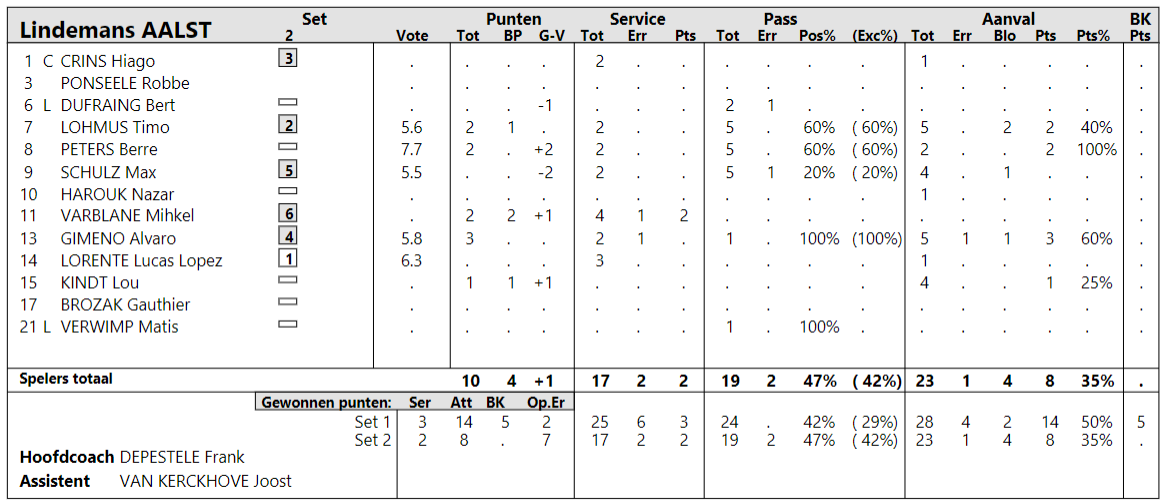
\includegraphics[width=\textwidth]{PL3_AM/SET2/PL3_AM_2.png}
  \caption{\label{fig:PL3_AM_2}Resultaten van de manuele invoer van Lindemans Aalst in set 2.}
\end{figure}

\begin{table}[ht!]
  \centering
  \scriptsize
  \begin{tabular}{|l|c|c|c|c|c|c|c|c|c|c|c|} \hline
    \textbf{Name} & SA & SE & TA & Pct & Eff & Rtg & 0 & 1 & 2 & 3 & ? \\ \hline
    Timo Lohmus & 0 & 0 & 1 & 1 & 0 & 2 &   & 1 &   & 0 &   \\
    Berre Peeters & 0 & 1 & 2 & 0.5 & -0.5 & 2.5 &   & 1 & 1 & 0 & 6 \\
    Max Schulz & 0 & 1 & 2 & 0.5 & -0.5 & 2.5 &   & 1 & 1 & 0 &   \\
    Nezar Harouk & 0 & 0 & 4 & 1 & 0 & 2.25 &   & 1 & 1 & 2 & 0 \\
    Mihkel Varblane & 1 & 1 & 4 & 0.75 & 0 & 1.33 & 1 & 1 &   & 1 & 0 \\
    Alvaro Gimeno Rubio & 0 & 3 & 3 & 0 & -1 & 3 &   &   & 3 & 0 &   \\
    Lucas Lorente López & 0 & 0 & 3 & 1 & 0 & 2 &   & 1 &   & 0 &   \\
    Bert Dufraing &   &   &   &   &   &   & 2 & 1 & 1 &   &   \\
    Matis Verwimp &   &   &   &   &   &   &   &   &   &   &   \\
    Lindemans Aalst & 1 & 7 & 25 & 0.72 & -0.24 & 2.36 & 1 & 4 & 5 & 15 & 0 \\
    Greenyard Maaseik & 1 & 6 & 19 & 0.68 & -0.26 & 2.25 & 1 & 2 & 5 & 8 & 0 \\ \hline
  \end{tabular}
  \caption[Serve statistieken gemaakt door Balltime AI voor Lindemans Aalst in set 2]{\label{tab:PL3ServeAalst2}Serve statistieken gemaakt door Balltime AI voor Lindemans Aalst in set 2.}
\end{table}

\begin{table}[ht!]
  \centering
  \scriptsize
  \begin{tabular}{|l|c|c|c|c|c|c|c|c|c|} \hline
    \textbf{Name} & 3 & 2 & 1 & 0 & TA & ? & Pass\% & Perfect PP\% & Good GP\% \\ \hline
    Timo Lohmus &   &   &   &   &   &   &   &   &   \\
    Berre Peeters & 4 & 2 &   & 12 & 12 & 0 & 2.33 & 0.5 & 0.83 \\
    Max Schulz &   & 1 &   & 1 & 1 & 0 & 0 & 0 & 0 \\
    Nezar Harouk &   &   &   &   &   &   &   &   &   \\
    Mihkel Varblane &   &   &   &   &   &   &   &   &   \\
    Alvaro Gimeno Rubio &   &   &   &   &   &   &   &   &   \\
    Lucas Lorente López &   &   &   &   &   &   &   &   &   \\
    Bert Dufraing & 2 & 1 & 1 &   & 4 & 0 & 2.25 & 0.5 & 0.75 \\
    Matis Verwimp &   &   &   &   &   &   &   &   &   \\
    Lindemans Aalst & 2 & 5 & 2 &   & 12 & 3 & 2 & 0.22 & 0.78 \\
    Greenyard Maaseik & 8 & 5 & 4 &   & 17 & 0 & 2.24 & 0.47 & 0.76 \\ \hline
  \end{tabular}
  \caption[Receive statistieken gemaakt door Balltime AI voor Lindemans Aalst in set 2]{\label{tab:PL3ReceiveAalst2}Receive statistieken gemaakt door Balltime AI voor Lindemans Aalst in set 2.}
\end{table}

\begin{table}[ht!]
  \centering
  \scriptsize
  \begin{tabular}{|l|c|c|c|c|c|c|c|} \hline
    \textbf{Name} & Set Ast & Set TA & Set SE & A/S & PCT & Dig DS & Dig DE \\ \hline
    Timo Lohmus &   &   &   &   &   &   &   \\
    Berre Peeters &   &   &   &   &   &   &   \\
    Max Schulz & 0 & 2 & 0 & 0 & 0 &   &   \\
    Nezar Harouk &   &   &   &   &   &   &   \\
    Mihkel Varblane &   &   &   &   &   &   &   \\
    Alvaro Gimeno Rubio &   &   &   &   &   &   &   \\
    Lucas Lorente López & 10 & 16 & 0 & 10 & 0.62 & 1 & 0 \\
    Bert Dufraing & 1 & 0 & 0 & 1 & 0 & 1 & 0 \\
    Matis Verwimp & 0 & 1 & 0 & 0 & 0 &   &   \\
    Lindemans Aalst & 12 & 19 & 0 & 12 & 0.63 & 9 & 1 \\
    Greenyard Maaseik & 10 & 20 & 0 & 10 & 0.5 & 5 & 0 \\ \hline
  \end{tabular}
  \caption[Setting en digging statistieken gemaakt door Balltime AI voor Lindemans Aalst in set 2]{\label{tab:PL3SetDigAalst2}Setting en digging statistieken gemaakt door Balltime AI voor Lindemans Aalst in set 2.}
\end{table}

\begin{table}[ht!]
  \centering
  \scriptsize
  \begin{tabular}{|l|c|c|c|c|c|c|c|c|c|} \hline
    \textbf{Name} & Attack K & E & TA & Atk\% & Kill\% & K/S & Error\% & Block BS & BA \\ \hline
    Timo Lohmus &   &   &   &   &   &   &   &   &   \\
    Berre Peeters & 1 & 7 & 4 & 1 & 0.57 & 4 & 0.14 &   &   \\
    Max Schulz & 2 & 1 & 5 & 0.2 & 0.4 & 2 & 0.2 &   &   \\
    Nezar Harouk &   &   &   &   &   &   &   &   &   \\
    Mihkel Varblane & 0 & 1 & 1 & -1 & 0 & 0 & 1 & 1 & 0 \\
    Alvaro Gimeno Rubio & 4 & 1 & 7 & 0.43 & 0.57 & 4 & 0.14 &   &   \\
    Lucas Lorente López & 0 & 0 & 1 & 0 & 0 & 0 & 0 & 0 & 0 \\
    Bert Dufraing &   &   &   &   &   &   &   &   &   \\
    Matis Verwimp &   &   &   &   &   &   &   &   &   \\
    Lindemans Aalst & 14 & 1 & 21 & 0.62 & 0.67 & 14 & 0.05 &   &   \\
    Greenyard Maaseik & 10 & 4 & 21 & 0.29 & 0.48 & 10 & 0.19 & 1 & 0 \\ \hline
  \end{tabular}
  \caption[Attacking en blocking statistieken gemaakt door Balltime AI voor Lindemans Aalst in set 2]{\label{tab:PL3AttBlockAalst2}Attacking en blocking statistieken gemaakt door Balltime AI voor Lindemans Aalst in set 2.}
\end{table}

\begin{figure}
  \centering
  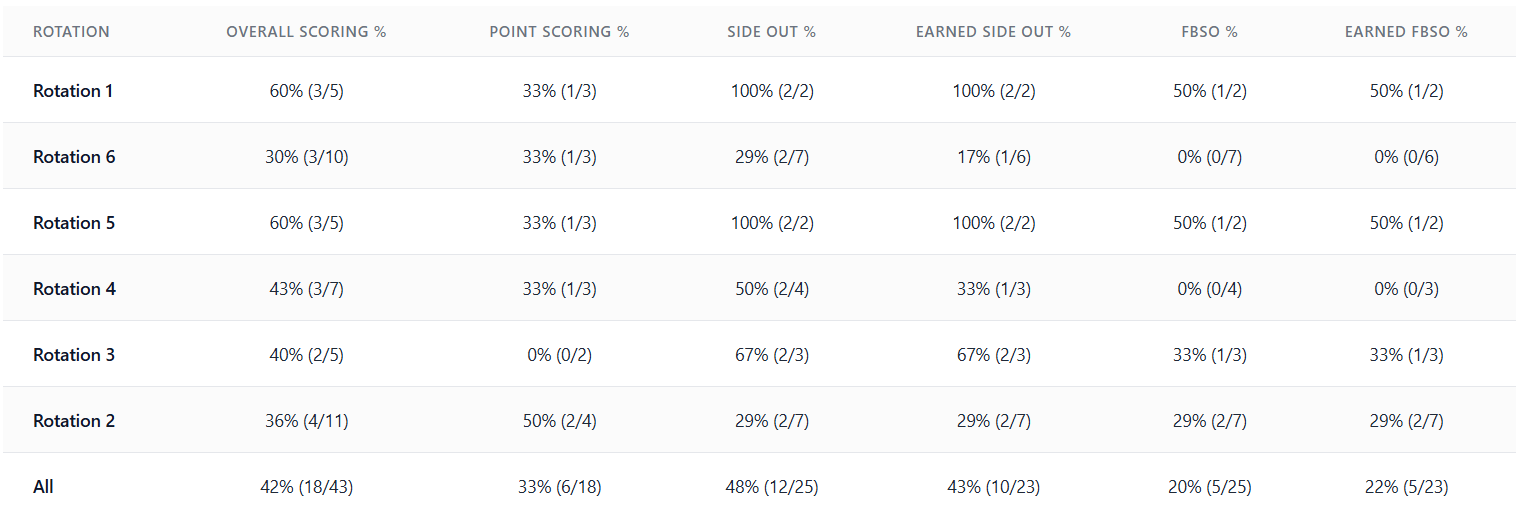
\includegraphics[width=\textwidth]{PL3_AM/SET2/ROT_STATS.png}
  \caption{\label{fig:PL3_ROT_STATS_2}Rotatie statistieken gemaakt door Balltime AI voor Lindemans Aalst in set 2.}
\end{figure}
\subsubsection{Set 3 - Greenyard Maaseik}
\label{sec:PL3_Greenyard3}

% TODO: tekst - stats OK

\begin{table}[ht!]
    \centering
    \scriptsize
    \begin{tabular}{|l|c|c|c|c|c|c|c|c|c|} \hline
        \textbf{Speler} & *E\% & Tot & = & / & - & ! & + & \#\\ \hline
        Samuel Fafchamps & 0\% & 3 &  &  & 3 &  &  &  \\ 
        Renet Vancker & 0\% & 1 &  &  & 1 &  &  & \\ 
        Jolan Cox & 25\% & 4 &  &  & 3 &  &  & 1 \\ 
        Dawid Pawlun & 50\% & 2 &  &  & 1 &  & 1 &  \\ 
        Miquel Angel Fornés & 25\% & 4 &  &  & 3 &  & 1 &  \\ 
        Hampus Ekstrand & 50\% & 4 & 1 &  &  &  & 2 & 1 \\ 
        Pierre Perin & 0\% & 2 & 1 &  &  &  & 1 &  \\ \hline
    \end{tabular}
    \caption[Manueel ingevoerde opslagstatistieken voor Greenyard Maaseik in set 3]{\label{tab:PL3ServeMaaseikMan3}Manueel ingevoerde opslagstatistieken voor Greenyard Maaseik in set 3.}
\end{table}

\begin{table}[ht!]
  \centering
  \scriptsize
  \begin{tabular}{|l|c|c|c|c|c|c|c|c|c|c|c|} \hline
    \textbf{Speler} & SA & SE & TA & Pct & Eff & Rtg & 0 & 1 & 2 & 3 \\ \hline
    Samuel Fafchamps &  &  & 3 & 100 & 0.00 & 2.67 &   &  & 1 & 2  \\
    Renet Vancker &  &  & 1 & 100 & 0.00 & 3.00 &  &  &  & 1 \\
    Jolan Cox & 1 &  & 4 & 100 & 0.25 & 1.50 & 1 & 1 & 1 & 1 \\
    Dawid Pawlun &  &  & 2 & 100 & 0.00 & 3.00 &   &   & & 1 \\
    Miquel Angel Fornés & 1 & 1 & 4 & 75 & 0.00 & 2.00 &   & 1 & 2 & 1 \\
    Hampus Ekstrand & 1 & 1 & 4 & 75 & 0.00 & 1.50 & 1 & 1 & 1 & 1\\
    Pierre Perin & & 1 & 2 & 50 & -0.50 & 2.5 &   &  & 1 & 1 \\ \hline
  \end{tabular}
  \caption[Opslagstatistieken gemaakt door Balltime AI voor Greenyard Maaseik in set 3]{\label{tab:PL3ServeMaaseikAI3}Opslag statistieken gemaakt door Balltime AI voor Greenyard Maaseik in set 3.}
\end{table}

% TODO: tekst - stats OK

\begin{table}[ht!]
    \centering
    \scriptsize
    \begin{tabular}{|l|c|c|c|c|c|c|c|c|c|} \hline
        \textbf{Speler} & *E\% & Tot & = & / & - & ! & + & \#\\ \hline
        Jolan Cox & -100\% & 1 & 1 &  &  &  &  & \\ 
        Landon Douglas Currie & 62\% & 8 &  &  & 1 & 2 & 1 & 4 \\ 
        Dawid Pawlun & -100\% & 1 &  & 1 &  &  &  &  \\ 
        Hampus Ekstrand & 100\% & 2 &  &  &  &  & 1 & 1 \\ 
        Pierre Perin & 38\% & 8 & 2 &  & 1 &  & 1 & 4 \\ \hline
    \end{tabular}
    \caption[Manueel ingevoerde receptiestatistieken voor Greenyard Maaseik in set 3]{\label{tab:PL3ReceiveMaaseikMan3}Manueel ingevoerde receptiestatistieken voor Greenyard Maaseik in set 3.}
\end{table}

\begin{table}[ht!]
  \centering
  \scriptsize
  \begin{tabular}{|l|c|c|c|c|c|c|c|c|c|} \hline
    \textbf{Speler} & 3 & 2 & 1 & 0 & TA & Pass\% & Perfect PP\% & Good GP\% \\ \hline
    Landon Douglas Currie & 3 & 3 & 2 &  & 8 & 2.12 & 38 & 75 \\
    Hampus Ekstrand & 1 & 1 &   & 2 & & 1.5 & 0 & 50 \\
    Pierre Perin & 6 & 1 &   & 2 & 9 & 2.22 & 67 & 78 \\ \hline
  \end{tabular}
  \caption[Receptiestatistieken gemaakt door Balltime AI voor Greenyard Maaseik in set 3]{\label{tab:PL3ReceiveMaaseikAI3}Receptiestatistieken gemaakt door Balltime AI voor Greenyard Maaseik in set 3.}
\end{table}

% TODO: tekst - stats OK

\begin{table}[ht!]
    \centering
    \scriptsize
    \begin{tabular}{|l|c|c|c|c|c|c|c|c|c|} \hline
        \textbf{Speler} & *E\% & Tot & = & / & - & ! & + & \#\\ \hline
        Renet Vancker & 100\% & 3 &  &  &  &  & 2 & 1 \\ 
        Dawid Pawlun & 100\% & 17 &  &  &  &  & 15 & 2 \\ 
        Pierre Perin & 100\% & 2 &  &  &  &  & 2 &  \\ \hline
    \end{tabular}
    \caption[Manueel ingevoerde spelverdelingsstatistieken gemaakt voor Greenyard Maaseik in set 3]{\label{tab:PL3SetMaaseikMan3}Manueel ingevoerde spelverdelingsstatistieken gemaakt voor Greenyard Maaseik in set 3.}
\end{table}

\begin{table}[ht!]
    \centering
    \scriptsize
    \begin{tabular}{|l|c|c|c|c|c|c|c|c|c|} \hline
        \textbf{Speler} & *E\% & Tot & = & / & - & ! & + & \#\\ \hline
        Samuel Fafchamps & 0\% & 1 & 1 &  &  &  &  &  \\ 
        Jolan Cox & 50\% & 2 & 1 & 1 &  &  &  & \\
        Landon Douglas Currie & 33\% & 3 & 1 &  & 1 &  & 1 &  \\
        Dawid Pawlun & 0\% & 3 & 2 &  & 1 &  &  &  \\ 
        Hampus Ekstrand & 100\% & 1 &  &  &  &  & 1 &\\ 
        Pierre Perin & 100\% & 1 &  &  &  &  & 1 & \\ \hline
    \end{tabular}
    \caption[Manueel ingevoerde verdedigingsstatistieken gemaakt voor Greenyard Maaseik in set 3]{\label{tab:PL3DigMaaseikMan3}Manueel ingevoerde verdedigingsstatistieken gemaakt voor Greenyard Maaseik in set 3.}
\end{table}

\begin{table}[ht!]
  \centering
  \scriptsize
    \begin{tabular}{|l|c|c|c|c|c|c|c|} \hline
    \textbf{Speler} & Ast & TA & SE & A/S & PCT & DS & DE \\ \hline
    Renet Vancker & 2 & 3 &  & 2.00 & 67 &   &   \\
    Landon Douglas Currie &  & 1 &  & 0.00 & 0 & 2 & 1 \\
    Dawid Pawlun & 8 & 17 & & 8.00 & 47 & 2 &  \\
    Hampus Ekstrand &  &  &  &  &  & 3 &  \\
    Pierre Perin &  & 2 &  & 0.00 & 0 & 1 &  \\ \hline
  \end{tabular}
  \caption[Spelverdelings- en verdedigingsstatistieken gemaakt door Balltime AI voor Greenyard Maaseik in set 3]{\label{tab:PL3SetDigMaaseikAI3}Spelverdelings- en verdedigingsstatistieken gemaakt door Balltime AI voor Greenyard Maaseik in set 3.}
\end{table}

% TODO: tekst  - stats OK

\begin{table}[ht!]
    \centering
    \scriptsize
    \begin{tabular}{|l|c|c|c|c|c|c|c|c|c|} \hline
        \textbf{Speler} & *E\% & Tot & = & / & - & ! & + & \#\\ \hline
        Samuel Fafchamps & 100\% & 1 &  &  &  &  &  & 1 \\ 
        Jolan Cox & 33\% & 12 &  & 2 &  & 1 & 3 & 6 \\ 
        Miquel Angel Fornés & 33\% & 3 &  & 1 &  &  &  & 2 \\ 
        Hampus Ekstrand & -50\% & 2 & 1 &  &  &  & 1 & \\ 
        Pierre Perin & -50\% & 4 & 3 &  &  &  &  & 1 \\ \hline
    \end{tabular}
    \caption[Manueel ingevoerde aanvalsstatistieken gemaakt Greenyard Maaseik in set 3]{\label{tab:PL3AttMaaseikMan3}Manueel ingevoerde aanvalsstatistieken gemaakt voor Greenyard Maaseik in set 3.}
\end{table}

\begin{table}[ht!]
    \centering
    \scriptsize
    \begin{tabular}{|l|c|c|c|c|c|c|c|c|c|} \hline
        \textbf{Speler} & *E\% & Tot & = & / & - & ! & + & \#\\ \hline
        Samuel Fafchamps & 33\% & 3 &  &  &  & 1 & 1 & 1 \\ 
        Jolan Cox & -75\% & 4 & 3 &  &  & 1 &  & \\ 
        Dawid Pawlun & -33\% & 3 & 1 &  & 1 & 1 &  &  \\ 
        Miquel Angel Fornés & -100\% & 1 & 1 &  &  &  &  & \\ 
        Hampus Ekstrand & 50\% & 2 &  &  &  & 1 &  & 1 \\  \hline
    \end{tabular}
    \caption[Manueel ingevoerde blokstatistieken gemaakt Greenyard Maaseik in set 3]{\label{tab:PL3BlockMaaseikMan3}Manueel ingevoerde blokstatistieken gemaakt voor Greenyard Maaseik in set 3.}
\end{table}

\begin{table}[ht!]
  \centering
  \scriptsize
  \begin{tabular}{|l|c|c|c|c|c|c|c|c|c|c|c|} \hline
    \textbf{Speler} & K & E & TA & Atk\% & Kill\% & K/S & Error\% & BS & BA & BE & B/S \\ \hline
    Samuel Fafchamps & 1 &  & 1 & 1.00 & 100 & 1 & 0 &  &   &  &  \\
    Jolan Cox & 6 & 2 & 12 & 0.33 & 50 & 6 & 17 &  &   &   & \\
    Dawid Pawlun &   &   &   &   &   &   &   & 1 & & & 1.00 \\
    Miquel Angel Fornés & 2 & 1 & 3 & 0.33 & 67 & 2 & 33 &  &   &  & \\
    Hampus Ekstrand &  & 1 & 2 & -0.50 & 0 &  & 50 & 1 & & & 1.00 \\
    Alex Saaremaa &  &  & 1 & 0.00 & 0 &  & 0 &  & & & \\
    Pierre Perin & 1 & 3 & 5 & -0.40 & 20 & 1 & 60 & &  & &  \\  \hline
  \end{tabular}
  \caption[Aanvals- en blokstatistieken gemaakt door Balltime AI voor Greenyard Maaseik in set 3]{\label{tab:PL3AttBlockMaaseikAI3}Aanvals- en blokstatistieken gemaakt door Balltime AI voor Greenyard Maaseik in set 3.}
\end{table}

\subsubsection{Set 4 - Lindemans Aalst}
\label{sec:PL3_Aalst4}

De opslagstatistieken zijn weergegeven in de tabel \ref{tab:PL3ServeAalstMan4} en \ref{tab:PL3ServeAalstAI4}. 

Bij de opslag komt het teken \# overeen met 0, + en / met 1, ! met 2, - en = met 3.

De foutieve opslagen, bij manuele invoer een = en bij AI-invoer een Serve Error (SE), zijn correct weergegeven.  Ook de perfecte opslag is hetzelfde. Bij de andere opslagen valt op dat de AI meer score 2 geeft en de manuele meer score 1.

\begin{table}[ht!]
    \centering
    \scriptsize
    \begin{tabular}{|l|c|c|c|c|c|c|c|c|}
        \hline
        \textbf{Speler} & *E\% & Tot & = & / & - & ! & + & \# \\ \hline
        Timo Lohmus & 100\% & 1 &  &  & & & 1 &  \\
        Berre Peters & -50\% & 2 & 1 &  & 1 &  & & \\ 
        Max Schulz & 0\% & 2 & 1 &  &  &  & 1 &\\ 
        Nezar Harouk & 50\% & 4 &  &  & 2 & & 2 &  \\ 
        Mihkel Varblane & 25\% & 4 & 1 &  & 1 &  & 1 & 1\\
        Alvaro Gimeno Rubio & -100\% & 3 & 3 &  &  &  &  & \\ 
        Lucas Lorente Lòpez & 33\% & 3 &  &  & 2 & & 1 &  \\ \hline
    \end{tabular}
    \caption[Manueel ingevoerde opslagstatistieken voor Lindemans Aalst in set 4]{\label{tab:PL3ServeAalstMan4}Manueel ingevoerde opslagstatistieken voor Lindemans Aalst in set 4.}
\end{table}

\begin{table}[ht!]
  \centering
  \scriptsize
  \begin{tabular}{|l|c|c|c|c|c|c|c|c|c|c|c|} \hline
    \textbf{Speler} & SA & SE & TA & Pct & Eff & Rtg & 0 & 1 & 2 & 3  \\ \hline
    Timo Lohmus &  &  & 1 & 100\% & 0.00 & 2.00 &   & &  1 &  \\
    Berre Peters &  & 1 & 2 & 50\% & -0.50 & 2.50 &   &  & 1 & 1 \\
    Max Schulz &  & 1 & 2 & 50\% & -0.50 & 2.50 &   &  & 1 & 1 \\
    Nezar Harouk &  &  & 4 & 100\% & 0.00 & 2.25 &   & 1 & 1 & 2 \\
    Mihkel Varblane & 1 & 1 & 4 & 75\% & 0.00 & 1.33 & 1 & 1 &   & 1 \\
    Alvaro Gimeno Rubio &  & 3 & 3 & 0\% & -1.00 & 3.00 &   &   &  & 3  \\
    Lucas Lorente Lòpez &  &  & 3 & 100\% & 0.00 & 2.00 &   &  &  1 &  \\\hline
  \end{tabular}
  \caption[Opslagstatistieken gemaakt door Balltime AI voor Lindemans Aalst in set 4]{\label{tab:PL3ServeAalstAI4}Opslagstatistieken gemaakt door Balltime AI voor Lindemans Aalst in set 4.}
\end{table}

De beoordeeldingen van de recepties zijn weergeven in tabel \ref{tab:PL3ReceiveAalstMan4} en \ref{tab:PL3ReceiveAalstAI4}.

De beoordeling van de receptie is op een andere wijze gedaan dan bij de manuele invoer. Bij de manuele invoer wordt er gebruik gemaakt van tekens, terwijl bij de AI-invoer gebruik wordt gemaakt van cijfers. Bij de receptie komt het teken \# overeen met 3, + en / met 2, ! met 1, - en = met 0.

De AI heeft bij geen enkele receptie een score van 0 gegeven. Bij de manuele invoer is dit wel het geval voor vijf recepties. Ook bij de andere scores wordt duidelijk dat de manuele invoer kritischer is dan de AI.

\begin{table}[ht!]
    \centering
    \scriptsize
    \begin{tabular}{|l|c|c|c|c|c|c|c|c|}
        \hline
        \textbf{Speler} & *E\% & Tot & = & / & - & ! & + & \# \\ \hline
        Bert Dufraing & 50\% & 4 &  &  & 1 & 1 & 1 & 1\\ 
        Berre Peters & 55\% & 11 & & 1 & 2 & 1 & 6 & 1 \\ 
        Max Schulz & -33\% & 3 & 1 &  & 1 & 1 &  & \\ \hline
    \end{tabular}
    \caption[Manueel ingevoerde receptiestatistieken voor Lindemans Aalst in set 4]{\label{tab:PL3ReceiveAalstMan4}Manueel ingevoerde receptiestatistieken voor Lindemans Aalst in set 4.}
\end{table}

\begin{table}[ht!]
  \centering
  \scriptsize
    \begin{tabular}{|l|c|c|c|c|c|c|c|c|c|} \hline
    \textbf{Speler} & 3 & 2 & 1 & 0 & TA & Pass\% & PP\% & GP\% \\ \hline
    Bert Dufraing & 2 & 1 & 1 &   & 4 & 2.25 & 50\% & 75\% \\  
    Berre Peters & 6 & 4 & 2 &  & 12 & 2.33 & 50\% & 83\% \\
    Max Schulz &   &  &  1 &  & 1 & 1.00 & 0\% & 0\% \\\hline
  \end{tabular}
  \caption[Receptiestatistieken gemaakt door Balltime AI voor Lindemans Aalst in set 4]{\label{tab:PL3ReceiveAalstAI4}Receptiestatistieken gemaakt door Balltime AI voor Lindemans Aalst in set 4.}
\end{table}

In tabel \ref{tab:PL3SetAalstMan4} en \ref{tab:PL3DigAalstMan4} zijn de manueel ingevoerde spelverdelings- en verdedigingsstatistieken weergegeven. De statistieken van de AI zijn weergegeven in tabel \ref{tab:PL3SetDigAalstAI4}.
Bij de spelverdelingsstatistieken valt op dat Max Schulz een actie meer heeft bij de AI-invoer dan bij de manuele invoer. Bij het bekijken van de video valt dan wel op dat hij effectief een actie meer heeft uitgevoerd. 

Bij de verdedigingsstatistieken zijn er verschillende hoeveelheden. Bij 2 van de spelers is het wel correct. Bij de andere is er een verschil van 2 tot 1 actie minder door de AI-invoer.

\begin{table}[ht!]
    \centering
    \scriptsize
    \begin{tabular}{|l|c|c|c|c|c|c|c|c|}
        \hline
        \textbf{Speler} & *E\% & Tot & = & / & - & ! & + & \# \\ \hline
        Bert Dufraing & 100\% & 1 &  &  &  & & 1 &  \\ 
        Max Schulz & 100\% & 1 &  &  &  & & & 1 \\ 
        Lucas Lorente Lòpez & 100\% & 16 &  &  &  &  & 15 & 1 \\ 
        Matis Verwimp &100\% & 1 & & & & & 1 & \\\hline
    \end{tabular}
    \caption[Manueel ingevoerde spelverdelingsstatistieken voor Lindemans Aalst in set 4]{\label{tab:PL3SetAalstMan4}Manueel ingevoerde spelverdelingsstatistieken voor Lindemans Aalst in set 4.}
\end{table}

\begin{table}[ht!]
    \centering
    \scriptsize
    \begin{tabular}{|l|c|c|c|c|c|c|c|c|}
        \hline
        \textbf{Speler} & *E\% & Tot & = & / & - & ! & + & \# \\ \hline
        Bert Dufraing & 50\% & 2 &  & 1 & 1 &  &  & \\ 
        Berre Peters & 50\% & 4 & 1 & 1 & 1 & & 1 &  \\ 
        Max Schulz & 0\% & 1 & 1 &  &  &  &  & \\ 
        Nezar Harouk & 0\% & 1 &  &  & 1 &  &  &  \\ 
        Lucas Lorente Lòpez & 0\% & 1 &  &  & 1 &  &  & \\ \hline
    \end{tabular}
    \caption[Manueel ingevoerde verdedigingsstatistieken voor Lindemans Aalst in set 4]{\label{tab:PL3DigAalstMan4}Manueel ingevoerde verdedigingsstatistieken voor Lindemans Aalst in set 4.}
\end{table}

\begin{table}[ht!]
  \centering
  \scriptsize
  \begin{tabular}{|l|c|c|c|c|c|c|c|} \hline
    \textbf{Speler} & Ast & TA & SE & PCT & DS &  DE \\ \hline
    Bert Dufraing &  & 1 &  & 0\% & 1 &  \\
    Berre Peters &   &   &   &   & 2 &   \\
    Max Schulz &  & 2 &  & 0\% &   &   \\
    Nezar Harouk &   &   &   &   &  1 &   \\
    Lucas Lorente Lòpez & 10 & 16 &  & 62\% & 1 &  \\
    Matis Verwimp &  & 1 & & 0\% &   &   \\ \hline
  \end{tabular}
 \caption[Spelverdelings- en verdedigingsstatistieken gemaakt door Balltime AI voor Lindemans Aalst in set 4]{\label{tab:PL3SetDigAalstAI4}Spelverdelings- en verdedigingsstatistieken gemaakt door Balltime AI voor Lindemans Aalst in set 4.}
\end{table}

De aanvalsstatistieken in deze set worden weergegeven in de tabellen \ref{tab:PL3AttAalstMan4} en \ref{tab:PL3AttBlockAalstAI4}. De blokstatistieken zijn weergegeven in de tabellen \ref{tab:PL3BlockAalstMan4} en \ref{tab:PL3AttBlockAalstAI4}. De AI-invoer geeft aan dat Lucas Lorente Lòpez ook één keer aanvalt, terwijl de manuele invoer dit niet aangeeft. Bij het bekijken van de video is duidelijk dat hij dit effectief niet doet. De hoeveelheid correcte aanvallen is bij beide hetzelfde aantal.

Bij de blokstatistieken is er een zeer groot verschil aanwezig. De AI geeft aan dat er maar één blok doorheen de hele set is, terwijl de manuele invoer er negen in totaal aangeeft.

De kwaliteit van aanvallen en blokkeringen worden niet beoordeeld door de AI. 

\begin{table}[ht!]
    \centering
    \scriptsize
    \begin{tabular}{|l|c|c|c|c|c|c|c|c|}
        \hline
        \textbf{Speler} & *E\% & Tot & = & / & - & ! & + & \# \\ \hline
        Berre Peters & 43\% & 7 & 1 &  &  & & 2 & 4 \\ 
        Max Schulz & 20\% & 5 & 1 &  & 1 & 1 & & 2 \\ 
        Mihkel Varblane & -100\% & 1 &  & 1 &  &  &  & \\ 
        Alvaro Gimeno Rubio & 43\% & 7 &  & 1 & & & 2 & 4 \\ \hline
    \end{tabular}
    \caption[Manueel ingevoerde aanvalsstatistieken voor Lindemans Aalst in set 4]{\label{tab:PL3AttAalstMan4}Manueel ingevoerde aanvalsstatistieken voor Lindemans Aalst in set 4.}
\end{table}

\begin{table}[ht!]
    \centering
    \scriptsize
    \begin{tabular}{|l|c|c|c|c|c|c|c|c|}
        \hline
        \textbf{Speler} & *E\% & Tot & = & / & - & ! & + & \# \\ \hline
        Max Schulz & -100\% & 1 & 1 &  &  &  &  & \\
        Nezar Harouk & -75\% & 4 & 3 & &  & 1 &  & \\ 
        Mihkel Varblane & -33\% & 3 & 2 &  &  & &  & 1 \\ 
        Alvaro Gimeno Rubio & -100\% & 1 & 1 &  &  &  &  & \\  \hline
    \end{tabular}
    \caption[Manueel ingevoerde blokstatistieken voor Lindemans Aalst in set 4]{\label{tab:PL3BlockAalstMan4}Manueel ingevoerde blokstatistieken voor Lindemans Aalst in set 4.}
\end{table}

\begin{table}[ht!]
  \centering
  \scriptsize
  \begin{tabular}{|l|c|c|c|c|c|c|c|c|c|c|c|} \hline
    \textbf{Speler} &  K & E & TA & Atk\% & Kill\% & Error\% & BS & BA & BE \\ \hline
    Berre Peters & 4 & 1 & 7 & 0.43 & 57\% & 14\% &  &  & \\
    Max Schulz & 2 & 1 & 5 & 0.20 & 40\% & 20\% &  &  & \\
    Mihkel Varblane &  & 1 & 1 & -1.00 & 0\% & 100\% & 1 & & \\
    Alvaro Gimeno Rubio & 4 & 1 & 7 & 0.43 & 57\% & 14\% &  &  & \\
    Lucas Lorente Lòpez &  &  & 1 & 0 & 0\% & 0\% &  &  &\\ \hline
  \end{tabular}
  \caption[Aanvals- en blokstatistieken gemaakt door Balltime AI voor Lindemans Aalst in set 4]{\label{tab:PL3AttBlockAalstAI4}Aanvals- en blokstatistieken gemaakt door Balltime AI voor Lindemans Aalst in set 4.}
\end{table}
